\documentclass{article}

\usepackage{tabularx}
\usepackage{changepage}
\usepackage{booktabs}
\usepackage{tikz}
\usepackage{caption}

\title{Problem Statement and Goals\\\progname}

\author{\authname}

\date{}

\input{../Comments}
%% Common Parts

\newcommand{\progname}{MTOBridge} % PUT YOUR PROGRAM NAME HERE
\newcommand{\authname}{Team 15, Alpha Software Solutions
\\ Badawy, Adham
\\ Yazdinia, Pedram
\\ Jandric, David
\\ Vakili, Farzad
\\ Vezina, Victor
\\ Chiu, Darren} % AUTHOR NAMES                  

\usepackage{hyperref}
    \hypersetup{colorlinks=true, linkcolor=blue, citecolor=blue, filecolor=blue,
                urlcolor=blue, unicode=false}
    \urlstyle{same}


\begin{document}

\maketitle

\begin{table}[hp]
\caption{Revision History} \label{TblRevisionHistory}
\begin{tabularx}{\textwidth}{llX}
\toprule
\textbf{Date} & \textbf{Developer(s)} & \textbf{Change}\\
\midrule
9/22/2022 & Pedram Yazdinida & First Draft\\
9/24/2022 & Pedram Yazdinida & First Revision\\
9/25/2022 & Pedram Yazdinida & Second Revision\\
\bottomrule
\end{tabularx}
\end{table}

\section{Problem Statement}

\subsection{Background}

For years, Bridge engineers in Ontario have based their bridge analysis on the Canadian Highway Bridge Design Code (CHBDC) (CSA S6-19) which typically features conservatism and adds excessive costs. With the development of refined methods of analysis, engineers can precisely determine the properties and constraints of the proposed design. Nevertheless, the new methods of analysis have yet to be offered within a one-stop program with an intuitive and simple UX. Using refined methods of analysis to precisely determine the load-carrying capacity of bridge members would allow bridge engineers to make well-informed decisions on bridge repair and load posting as well. 
 
\subsection{Problem}

As part of a direct collaboration with Ontario Ministry of Transport, the proposed solution will take advantage of the refined methods of analysis developed by the Department of Civil Engineering to create a full-fledged application that can easily elevate the computations done by Bridge Engineers. MTOBridge will package the existing engine written in MATLAB with modern interactive User Interface (UI), well-defined Input/Output (I/O), and standard bridge section Database. The program will allow engineers to intuitively input their specifications on load, material, geometry, and prestress where the engine is then used to solve for variables on ultimate flexure, shear and torsion. The user will have the ability to switch between the refined and traditional methods of analysis, visualizing the cost savings and improvements across the board. Finally, the output will also include interactable graphs and charts where the user can find further specific information based on a given point. 


\subsection{Inputs and Outputs}

%\wss{Characterize the problem in terms of ``high level'' inputs and outputs.  
%Use abstraction so that you can avoid details.}


\tikzset{every picture/.style={line width=0.75pt}} %set default line width to 0.75pt   

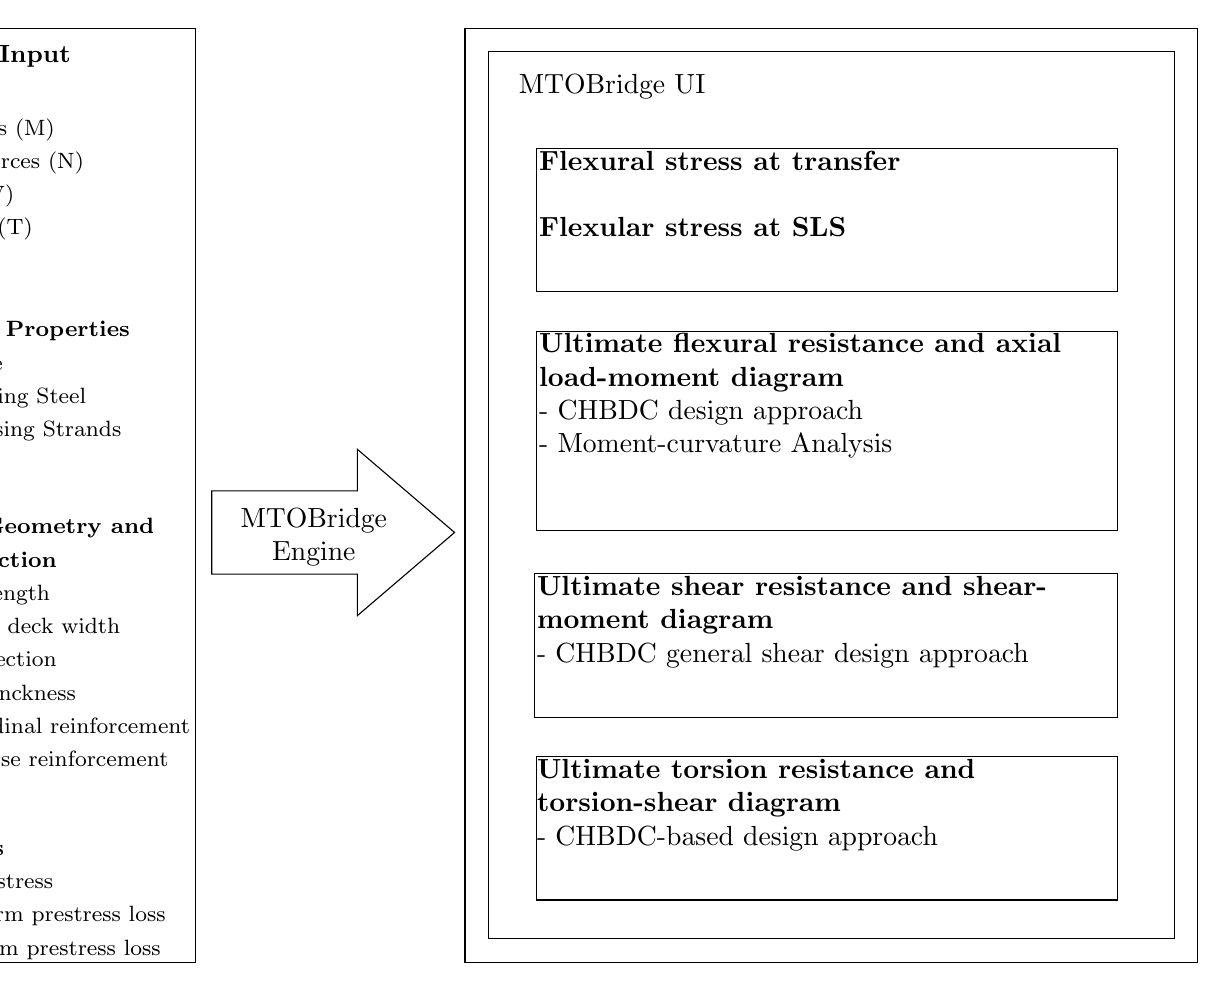
\begin{tikzpicture}[x=0.75pt,y=0.75pt,yscale=-1,xscale=1,trim left=2cm]
%\path (200,200); %set diagram left start at 0, and has height of 554

%Shape: Rectangle [id:dp40713623006932687] 
\draw   (9.8,30) -- (156.55,30) -- (156.55,480) -- (9.8,480) -- cycle ;
%Right Arrow [id:dp022223857966380267] 
\draw   (164.55,252.93) -- (234.75,252.93) -- (234.75,232.91) -- (281.55,272.95) -- (234.75,313) -- (234.75,292.98) -- (164.55,292.98) -- cycle ;
%Shape: Rectangle [id:dp6440046928241534] 
\draw   (321,87.9) -- (601,87.9) -- (601,157) -- (321,157) -- cycle ;
%Shape: Rectangle [id:dp15284232981487356] 
\draw   (321,175.9) -- (601,175.9) -- (601,272) -- (321,272) -- cycle ;
%Shape: Rectangle [id:dp9132870930202315] 
\draw   (320,292.9) -- (601,292.9) -- (601,362) -- (320,362) -- cycle ;
%Shape: Rectangle [id:dp5415191968439061] 
\draw   (321,380.9) -- (601,380.9) -- (601,450) -- (321,450) -- cycle ;

%Shape: Frame [id:dp281589755928753] 
\draw   (286.55,30) -- (639.55,30) -- (639.55,480) -- (286.55,480) -- cycle(628.23,41.32) -- (297.86,41.32) -- (297.86,468.68) -- (628.23,468.68) -- cycle ;

\draw (60.8,36.81) node [anchor=north west][inner sep=0.75pt]   [align=left] {\textbf{{\small Input}}};
% Text Node
\draw (11.8,56.81) node [anchor=north west][inner sep=0.75pt]   [align=left] {\textbf{{\footnotesize Loads}}\\{\footnotesize - Moments (M) }\\{\footnotesize - Axial Forces (N)}\\{\footnotesize - Shear (V)}\\{\footnotesize - Torsion (T)}};
% Text Node
\draw (11,170) node [anchor=north west][inner sep=0.75pt]   [align=left] {\textbf{{\footnotesize Material Properties}}\\{\footnotesize - Concrete}\\{\footnotesize - Reinforcing Steel}\\{\footnotesize - Prestressing Strands}\\};
% Text Node
\draw (11,265) node [anchor=north west][inner sep=0.75pt]   [align=left] {\textbf{{\footnotesize Girder Geometry and }}\\\textbf{{\footnotesize Cross Section}}\\{\footnotesize - Girder length }\\{\footnotesize - Effective deck width}\\{\footnotesize - Girder section}\\{\footnotesize - Deck thinckness}\\{\footnotesize - Longitudinal reinforcement}\\{\footnotesize - Transverse reinforcement}};
% Text Node
\draw (11,420) node [anchor=north west][inner sep=0.75pt]   [align=left] {\textbf{{\footnotesize Prestress}}\\{\footnotesize - Jacking stress }\\{\footnotesize - Short-term prestress loss}\\{\footnotesize - Long-term prestress loss}};
% Text Node
\draw (176,260) node [anchor=north west][inner sep=0.75pt]   [align=left] {\begin{minipage}[lt]{54.67pt}\setlength\topsep{0pt}
\begin{center}
MTOBridge\\Engine
\end{center}

\end{minipage}};
% Text Node
\draw (311,51) node [anchor=north west][inner sep=0.75pt]   [align=left] {\begin{minipage}[lt]{67.71pt}\setlength\topsep{0pt}
\begin{center}
MTOBridge UI
\end{center}

\end{minipage}};
% Text Node
\draw (320,381.09) node [anchor=north west][inner sep=0.75pt]   [align=left] {\textbf{Ultimate torsion resistance and}\\\textbf{torsion-shear diagram} \\\mbox{-} CHBDC-based design approach };
% Text Node
\draw (320,292.9) node [anchor=north west][inner sep=0.75pt]   [align=left] {\textbf{Ultimate shear resistance and shear-}\\\textbf{moment diagram}\\\mbox{-} CHBDC general shear design approach \\};
% Text Node
\draw (321,175.9) node [anchor=north west][inner sep=0.75pt]   [align=left] {\textbf{Ultimate flexural resistance and axial }\\\textbf{load-moment diagram}\\\mbox{-} CHBDC design approach \ \\\mbox{-} Moment-curvature Analysis };
% Text Node
\draw (321,87.9) node [anchor=north west][inner sep=0.75pt]   [align=left] {\textbf{Flexural stress at transfer }\\\\\textbf{Flexular stress at SLS}};


\end{tikzpicture}

\captionof{figure}{\textbf{MTOBridge Data Flow}}

\subsection{Stakeholders}

\begin{itemize}
  \item Ontario Ministry of Transport
	\begin{itemize}
	\item{The proposed porgram will be primary used by Engineers within Ontario Minstry of Transport. }
	\end{itemize}
  \item Department of Civil Engineering, McMaster
		\begin{itemize}
	\item{The proposed porgram will be directly developed in collaboration with Department of Civil Eningeering. }
		\end{itemize}
  \item Department of Software Engineering, McMaster 
		\begin{itemize}
	\item{The proposed program will be directly developed by Engineers from the Department of Software and Computing.} 
		\end{itemize}
\end{itemize}
\subsection{Environment}
\begin{itemize}
  \item Compatible with the latest Windows 10 versions (20H1+)
  \item Fully operational offline 
  \item Requires C++ GNU compiler 
\end{itemize}
%\wss{Hardware and software}

\section{Goals}

\subsection {Interactive UI}

\subsection {Ease of Use}

\subsection {Graphic Output}

\subsection {Cost Savings}

\subsection {Visualizing the Improvements}

\section{Stretch Goals}

\subsection {in-App Sketch function}

\subsection {Customizable UI}

\end{document}